\documentclass[aspectratio=169, 11pt]{beamer}

\usetheme{metropolis}
\usepackage{appendixnumberbeamer}
\usepackage{booktabs}
\usepackage{graphicx}
\usepackage{xcolor}
\usepackage{tikz}
\usepackage{listings}
\usepackage{amsmath}
\usepackage{multirow}

% Lean / Python listings
\lstdefinestyle{lean}{
    basicstyle=\ttfamily\scriptsize,
    keywordstyle=\color{blue!70!black}\bfseries,
    commentstyle=\color{green!50!black},
    showstringspaces=false,
    breaklines=true,
    frame=single,
    backgroundcolor=\color{gray!5},
    rulecolor=\color{gray!30},
}

% Cambridge-inspired palette
\definecolor{camblue}{HTML}{003E74}
\definecolor{camlightblue}{HTML}{5790AB}
\definecolor{camgreen}{HTML}{1E6F5C}
\definecolor{camgrey}{HTML}{7A8B99}
\definecolor{camlightgrey}{HTML}{E8ECF0}
\definecolor{camred}{HTML}{A31F34}

\setbeamercolor{frametitle}{bg=camblue, fg=white}
\setbeamercolor{title}{fg=camblue}
\setbeamercolor{progress bar}{fg=camgreen}
\setbeamercolor{alerted text}{fg=camred}

\setbeamerfont{title}{size=\Large, series=\bfseries}
\setbeamerfont{frametitle}{size=\large}
\setbeamertemplate{navigation symbols}{}

\title{Mode Collapse in RL-Trained\\Theorem Provers}
\subtitle{Structural Guidance as a Diagnostic and Remedy}
\author{Zachary Burton}
\institute{MIT $\to$ MPhil in Advanced Computer Science, Cambridge}
\date{arXiv: 2601.16172}

\begin{document}

% ============================================================
\begin{frame}[plain]
  \maketitle
\end{frame}

% ============================================================
\begin{frame}{Background: Neural Theorem Proving}
\begin{columns}[T]
\begin{column}{0.55\textwidth}
\textbf{Setup:}
\begin{itemize}
    \item Formal theorem $x$ in Lean 4
    \item LLM $P_\theta$ generates tactic proof $y$
    \item Lean kernel verifies: $\text{check}(x, y) \in \{\top, \bot\}$
    \item Sample $k$ attempts, accept if any verify
\end{itemize}

\vspace{0.4em}
\textbf{Model:} DeepSeek-Prover-V1.5-RL
\begin{itemize}
    \item 7B params, GRPO-trained (SFT $\to$ RL)
    \item Evaluated on miniF2F: 244 competition-level theorems
    \item Pinned to Lean v4.9.0-rc1 (training env)
\end{itemize}
\end{column}
\begin{column}{0.38\textwidth}
\centering
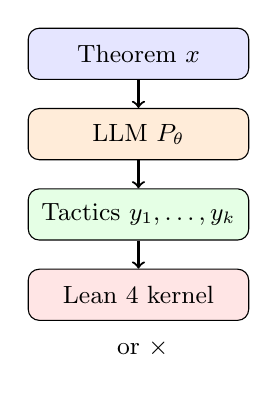
\begin{tikzpicture}[
    box/.style={draw, rounded corners, minimum width=2.8cm, minimum height=0.65cm, align=center, font=\small},
    scale=0.85
]
    \node[box, fill=blue!10] (thm) at (0, 3) {Theorem $x$};
    \node[box, fill=orange!15] (llm) at (0, 1.8) {LLM $P_\theta$};
    \node[box, fill=green!10] (tac) at (0, 0.6) {Tactics $y_1, \ldots, y_k$};
    \node[box, fill=red!10] (lean) at (0, -0.6) {Lean 4 kernel};
    \node[font=\small] at (0, -1.4) {$\checkmark$ or $\times$};
    \draw[->, thick] (thm) -- (llm);
    \draw[->, thick] (llm) -- (tac);
    \draw[->, thick] (tac) -- (lean);
\end{tikzpicture}
\end{column}
\end{columns}
\end{frame}

% ============================================================
\begin{frame}{Hypothesis: Mathematical Intuition Should Help}

\begin{columns}[T]
\begin{column}{0.48\textwidth}
\textbf{The core idea:}\\[0.3em]
A human mathematician knows that some problems want induction, others want contradiction, others want algebraic simplification.

\vspace{0.4em}
RL-trained LLMs lack this intuition. They converge on a narrow default strategy and repeat it---even when it fails.

\vspace{0.4em}
\textbf{If we inject a mathematician's sense of ``how to attack this,'' the model should do better.}
\end{column}
\begin{column}{0.48\textwidth}
\textbf{Evidence---sampling saturates:}

\vspace{0.3em}
\begin{tabular}{@{}lcc@{}}
\toprule
Budget & Solved & $\Delta$ \\
\midrule
$k=16$ & 38 / 244 & --- \\
$k=32$ & 42 / 244 & +4 \\
$k=64$ & \alert{42 / 244} & \alert{+0} \\
\bottomrule
\end{tabular}

\vspace{0.4em}
Doubling the budget: \alert{zero new proofs}.\\[0.3em]
The model isn't exploring---it's stuck. More compute alone won't fix this. \emph{Mathematical guidance} might.
\end{column}
\end{columns}
\end{frame}

% ============================================================
\begin{frame}{Method: Expert Hints as Tactic Prefixes}

\textbf{Idea:} Encode a mathematician's intuition as a tactic prefix---tell the model \emph{how to start} the proof.

\vspace{0.2em}
$P_\theta(y \mid x, s)$: model completes proof of theorem $x$ given hint $s$.

\vspace{0.3em}
\begin{columns}[T]
\begin{column}{0.42\textwidth}
\textbf{15 hints} reflecting common strategies:
\vspace{0.2em}

{\small
\begin{tabular}{@{}rl@{}}
0. & (empty --- no hint) \\
1. & \texttt{simp} \\
2. & \texttt{intro} \\
3. & \texttt{intros} \\
4. & \texttt{constructor} \\
5. & \texttt{refine ?\_} \\
6. & \texttt{norm\_num} \\
7. & \texttt{linarith} \\
\end{tabular}
\hspace{0.3em}
\begin{tabular}{@{}rl@{}}
8. & \texttt{nlinarith} \\
9. & \texttt{ring} \\
10. & \texttt{ring\_nf} \\
11. & \texttt{aesop} \\
12. & \texttt{refine $\langle$?\_,?\_$\rangle$} \\
13. & \texttt{simp; try aesop} \\
14. & \texttt{simp; try nlinarith} \\
& \\
\end{tabular}
}
\end{column}
\begin{column}{0.54\textwidth}
\textbf{The analogy:}\\[0.3em]
A student comes to you stuck on a proof. You don't solve it for them---you say ``have you tried induction?'' or ``what if you simplify first?''

\vspace{0.5em}
That small nudge is often enough. The model can \emph{execute} tactics well; it just picks the wrong \emph{strategy}.

\vspace{0.5em}
\textbf{Properties:}
\begin{itemize}
    \item No retraining, no tree search
    \item Compatible with any completion-based prover
\end{itemize}
\end{column}
\end{columns}
\end{frame}

% ============================================================
\begin{frame}[fragile]{Concrete Example: Hints Unlock New Proofs}

\textbf{Prove} $12 \mid 4^{n+1} + 20$.
\quad {\small Without hint: model tries \texttt{norm\_num} variants, fails all 16 attempts.}

\vspace{0.3em}
\begin{columns}[T]
\begin{column}{0.48\textwidth}
Hint \texttt{simp} $\to$ model completes:
\begin{lstlisting}[style=lean]
theorem induction_12dvd4expnp1p20
  (n : N) : 12 | 4^(n+1) + 20 := by
  simp
  induction n with
  | zero => simp
  | succ n ih =>
    simp_all [Nat.mul_mod,
              Nat.pow_succ]
    omega
\end{lstlisting}
{\scriptsize The hint nudged the model toward \texttt{simp} + \texttt{induction}---a strategy it never tried on its own.}
\end{column}
\begin{column}{0.48\textwidth}
\textbf{Another:} $ab{=}180$, $2(a{+}b){=}54 \Rightarrow a^2{+}b^2{=}369$

\vspace{0.2em}
{\small Without hint: tries \texttt{field\_simp}, loops, fails.}

\vspace{0.2em}
Hint \texttt{ring} $\to$ model completes:
\begin{lstlisting}[style=lean]
theorem mathd_algebra_141
  (a b : R)
  (h1 : a * b = 180)
  (h2 : 2 * (a + b) = 54) :
  a^2 + b^2 = 369 := by
  ring
  nlinarith
\end{lstlisting}

\vspace{0.3em}
{\small 13 theorems solved \textbf{only} via hints (never by i.i.d.\ sampling).}
\end{column}
\end{columns}
\end{frame}

% ============================================================
\begin{frame}{Results + Ablation}

\begin{columns}[T]
\begin{column}{0.46\textwidth}
\textbf{Main results:}

\vspace{0.2em}
{\small
\begin{tabular}{@{}lccc@{}}
\toprule
& @16 & @32 & @64 \\
\midrule
i.i.d.\ baseline & 38 & 42 & 42 \\
\textbf{skeleton hints} & \textbf{55} & \textbf{58} & \textbf{60} \\
\midrule
Relative gain & +45\% & +38\% & +43\% \\
\bottomrule
\end{tabular}
}

\vspace{0.3em}
Baseline \textbf{flatlines} ($42 \to 42$).\\
Hints \textbf{keep climbing} ($55 \to 58 \to 60$).
\end{column}
\begin{column}{0.50\textwidth}
\textbf{Ablation} (Pass@16): is \emph{any} perturbation enough?

\vspace{0.2em}
{\small
\begin{tabular}{@{}lcc@{}}
\toprule
Condition & Solved & vs.\ base \\
\midrule
C2: random tokens & 25 & \alert{$-34\%$} \\
A: i.i.d.\ (control) & 38 & --- \\
C1: paraphrases & 38 & $\pm 0\%$ \\
\textbf{B: tactic hints} & \textbf{55} & \textbf{$+45\%$} \\
\bottomrule
\end{tabular}
}

\vspace{0.3em}
Collapse is in \emph{tactic selection}, not instruction following. Only structural hints help.
\end{column}
\end{columns}
\end{frame}

% ============================================================
\begin{frame}{Base vs.\ RL: RL Creates Capability and Collapses It}

\begin{columns}[T]
\begin{column}{0.48\textwidth}
Same architecture, same pre-training---with and without GRPO.

\vspace{0.3em}
\begin{tabular}{@{}lcccc@{}}
\toprule
& @16 & @32 & @64 & Hint effect \\
\midrule
BASE i.i.d. & 0 & 0 & 0 & \multirow{2}{*}{None} \\
BASE hints & 0 & 0 & 0 & \\
\midrule
RL i.i.d. & 38 & 42 & 42 & \multirow{2}{*}{\textbf{+43\%}} \\
RL hints & 55 & 58 & 60 & \\
\bottomrule
\end{tabular}

\vspace{0.3em}
Base model outputs \texttt{sorry} for every theorem---\textbf{zero proof capability}.
\end{column}
\begin{column}{0.48\textwidth}
\textbf{The narrative:}
\begin{enumerate}
  \item RL \emph{creates} proof capability\\(BASE $\to$ RL: $0 \to 38+$)
  \item RL simultaneously \emph{narrows} the strategy space (mode collapse)
  \item Structural hints recover diversity that RL eliminates
\end{enumerate}

\vspace{0.4em}
\textbf{Broader point:} RL gives the model \emph{skill} but not \emph{judgment}. Mathematical experts can supply the judgment that RL strips away.
\end{column}
\end{columns}
\end{frame}

% ============================================================
\begin{frame}{Directions at Cambridge}

\begin{columns}[T]
\begin{column}{0.48\textwidth}
\textbf{Research proposal:} studying \textbf{proof search itself}---how proof states evolve, how tactic sequences branch via subgoal decomposition, and how RL and verifier feedback shape exploration.

\vspace{0.4em}
\textbf{Open questions:}
\begin{itemize}
  \item What forms of expert guidance help most? (tactic-level, lemma-level, strategic?)
  \item Can we \emph{learn} to select hints from proof structure? (hint retrieval)
  \item Can RL preserve mathematical judgment, not just maximize reward?
\end{itemize}
\end{column}

\begin{column}{0.48\textwidth}
\textbf{Planned modules:}
\begin{itemize}
  \item L81 (Proof Assistants)
  \item L313 (HoTT \& Univalent Foundations)
  \item L330 (Quantum Complexity Theory)
  \item R252 (Deep Learning Theory)
\end{itemize}

\vspace{0.4em}
\textbf{Paper status:} Targeting AI4Math @ ICML 2026

\vspace{0.2em}
\centering
\texttt{arXiv:2601.16172}
\end{column}
\end{columns}
\end{frame}

\end{document}
